\documentclass{article}
\usepackage[T1]{fontenc}
\usepackage{lmodern}
\usepackage{graphicx}
\usepackage{amsmath,amssymb}
\usepackage[a4paper,margin=2cm]{geometry}
\usepackage[absolute,overlay]{textpos}
\setlength{\TPHorizModule}{1mm}
\setlength{\TPVertModule}{1mm}
\usepackage[indonesian]{babel}
\usepackage{hyperref}
\setlength{\emergencystretch}{2em}
% unit: Halaman 13

\begin{document}

% === Halaman 13 (llm) ===

Matriks permutasi kompresi PC-1:

\vspace{10mm}

\textcolor{red}{Perhatikan, bit-bit parity, yaitu bit ke-8, 16, 28, ... dibuang, sehingga menjadi 56 bit}

\vspace{40mm}

$C_0$: berisi bit-bit dari $K$ pada posisi

\[
\begin{aligned}
&57, 49, 41, 33, 25, 17, 9, 1, 58, 50, 42, 34, 26, 18 \\
&10, 2, 59, 51, 43, 35, 27, 19, 11, 3, 60, 52, 44, 36
\end{aligned}
\]

$D_0$: berisi bit-bit dari $K$ pada posisi

\[
\begin{aligned}
&63, 55, 47, 39, 31, 23, 15, 7, 62, 54, 46, 38, 30, 22 \\
&14, 6, 61, 53, 45, 37, 29, 21, 13, 5, 28, 20, 12, 4
\end{aligned}
\]

% deskripsi: Tabel matriks permutasi kompresi PC-1 yang berisi angka-angka posisi bit.
% bbox normalisasi: [0.0600, 0.1080, 0.9400, 0.5020]
\begin{textblock*}{184.80mm}(12.60mm,32.08mm)
\noindent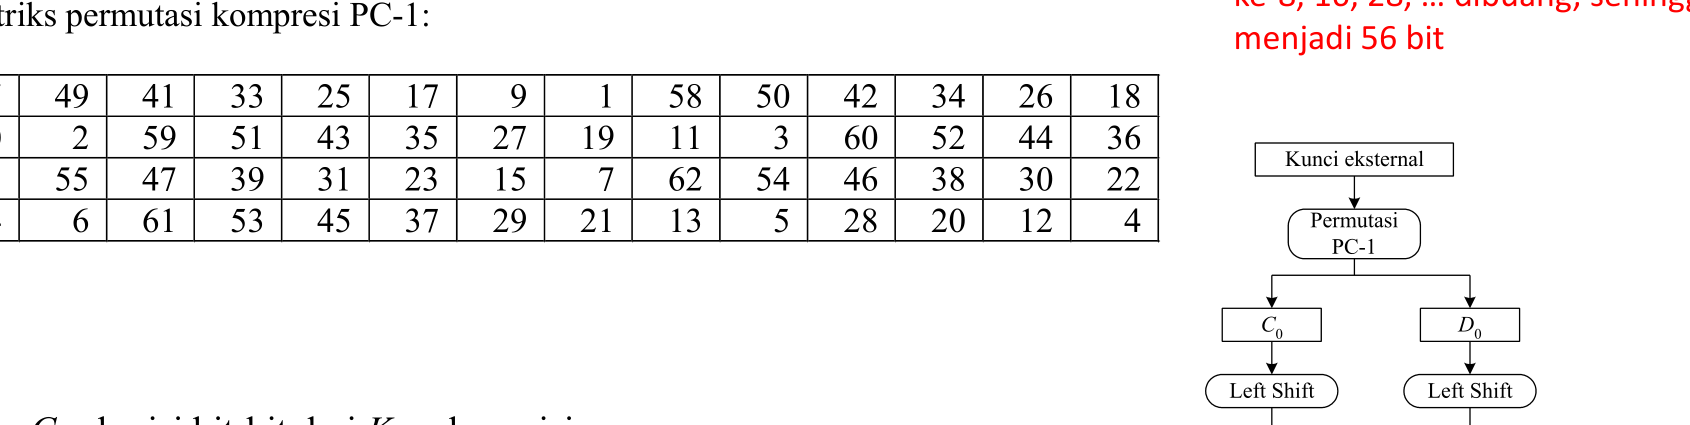
\includegraphics[width=184.80mm,height=117.02mm]{../../images/llm/page_013_img_01.png}%
\end{textblock*}

% deskripsi: Diagram alur proses penjadwalan kunci (key scheduling) DES, menunjukkan penggunaan Permutasi PC-1, Left Shift, dan Permutasi PC-2 untuk menghasilkan subkey K1 sampai K16.
% bbox normalisasi: [0.0600, 0.5180, 0.9400, 0.9120]
\begin{textblock*}{184.80mm}(12.60mm,153.85mm)
\noindent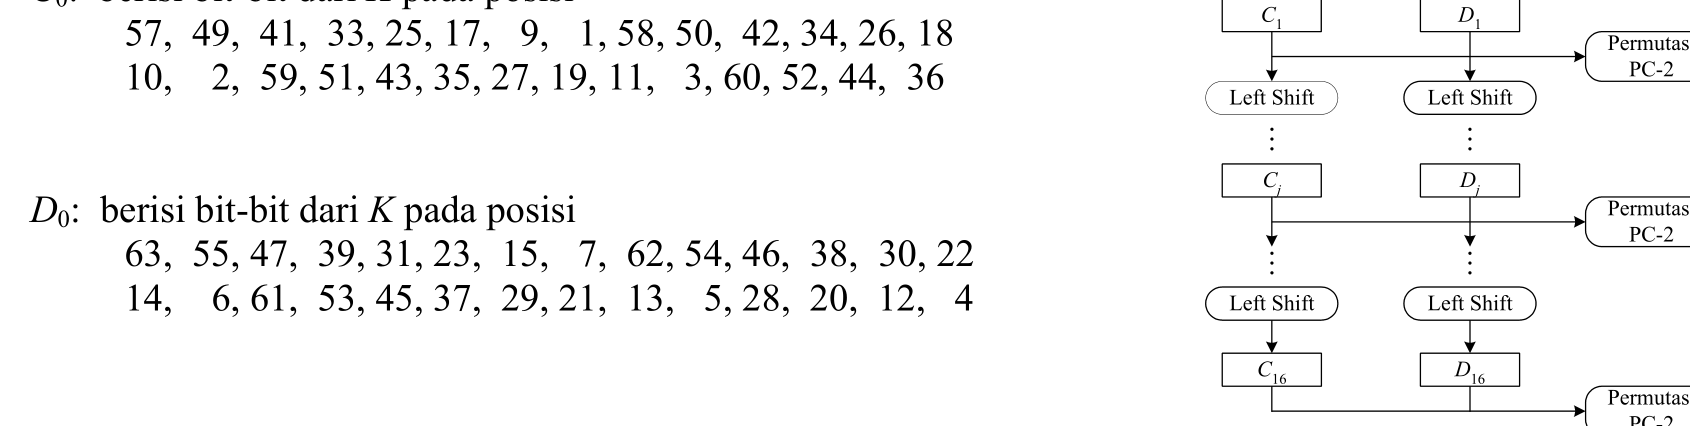
\includegraphics[width=184.80mm,height=117.02mm]{../../images/llm/page_013_img_02.png}%
\end{textblock*}

% bbox perkiraan otomatis: Tabel matriks permutasi kompresi PC-1 yang berisi angka-angka posisi bit.
% bbox perkiraan otomatis: Diagram alur proses penjadwalan kunci (key scheduling) DES, menunjukkan penggunaan Permutasi PC-1, Left Shift, dan Permutasi PC-2 untuk menghasilkan subkey K1 sampai K16.

\end{document}
